\section{Four new layouts: paired full-posterior forecast study}
This study replaces only the template-area predictor while retaining the full original geometric bank and quadrature. It is distinct from the earlier conditional-mean/fine-basis probe. All twenty-four short branches and eight complete episodes are retained, including censored coverage. Neutral/category short re-rankings hold fitted geometry, instance associations, and the frontend fixed and intervene only on the structural prior. The complete matrix compares two forecasts under S, not a full G/S semantic-frontend removal.
\subsection{Paired Forecast Selection in Unseen Layouts}
\label{sec:paired-forecast-layouts}

\paragraph{Comparison Question.}
We test whether a forecast that explicitly simulates future RGB-D acquisition selects a route that reconstructs more object surface than the visibility-based forecast. Both forecasts use the same geometry fitted from the acquired prefix, the same full geometric and structural posterior, the same category cues, and the same original surface quadrature. The only replaced term is predicted template-surface gain. The unknown-coverage and measured-surface scores, route costs, and execution rules remain shared. Hypothetical surfaces are used for prediction and are never fused into the measured reconstruction.

\paragraph{Layouts and Observations.}
Four layouts combine two furniture arrangements for each of two room-connectivity topologies: a four-room chain and a four-room cycle. Dimensions, doorway positions, furniture positions, and furniture orientations differ across the layouts. The layouts reuse the open-shelf and closed-cabinet assets used in development; thus, this experiment tests new spatial arrangements and topologies, rather than unseen CAD categories or natural-scene generalization. The simulator supplies exact poses, noiseless opaque RGB-D observations, and ideal visible category and instance labels. A fixed scripted acquisition history defines two decision states per layout. These states are controlled replay checkpoints, not autonomous prefix trajectories or independent scenes.

\paragraph{Matched Candidate Routes.}
Before evaluating either forecast, we group the original candidate routes by outbound action count. We retain the largest group whose action counts differ by at most three, resolving ties by the lower cost band and then candidate identifiers. The three evaluated routes include the visibility and acquisition forecasts' respective selections under the category prior; any remaining slot is filled by candidate identifier. All four combinations of forecast and neutral/category prior are then ranked on this same three-route set. The best measured route refers only to these three routes. This matching applies to the short-branch diagnostic; complete policy episodes retain every candidate produced by the inherited planner.

\paragraph{Prefix Preparation.}
Two originally frozen chain-layout checkpoints initially lacked three cost-close routes in the prescribed cost band. Before any new forecast score or branch outcome was evaluated, the preparation protocol was amended to advance only these two checkpoints along their existing acquisition scripts. The earliest checkpoint with three eligible routes was used: Chain~A p1 advances from 17 to 24 paid actions and Chain~B p1 from 17 to 20, with a separation of at least four actions from each second checkpoint. The original preparation failures, all intervening cost-only checks, the other six checkpoints, and the four source layouts are retained. This amendment changes controlled acquisition prefixes and does not modify the complete exploration policy.

\paragraph{Measured Outcome.}
Each route is executed once from an identical copy of its acquired prefix. Both forecasts are evaluated against this shared actual branch record. We measure object surface using fixed, independently sampled reference points from the source shelf and cabinet surfaces that are visible from the reference camera lattice. For reference point $i$, let $w_i$ be its surface-area weight and $b_i$ and $a_i$ indicate whether the measured native TSDF lies within $5\,$cm before and after the branch. Gross-new, lost, and net surface are
\begin{equation}
 A_{+}=\sum_i w_i(1-b_i)a_i,\qquad
 A_{-}=\sum_i w_i b_i(1-a_i),\qquad
 A_{\mathrm{net}}=A_{+}-A_{-}.
\end{equation}
The primary selection metric is $A_{+}$ for the chosen route; lost and net area are retained to expose reconstruction changes that gross gain alone would hide. Reference geometry is opened only by the independent evaluator after predictions and actual branches are recorded. We also report the chosen route's gap to the best of three, prediction mean absolute error, unchanged selections, failures, and recorded execution time. Missing measurements remain missing; partial execution is retained with its actual measured surface and completion status.

\paragraph{Complete Exploration Comparison.}
After the first twelve branches are tabulated and the remaining twelve are evaluated, each forecast is run once in every layout with the category prior. The eight complete episodes share initial observations, geometry inference, sensing, candidates, and a budget of $256$ paid actions including return. We report source-referenced object recall and whole-scene surface F1 at $5\,$cm, actions to $95\%$ and $100\%$ correct-free coverage, path length, collisions, and return status. Correct-free coverage uses the source start-reachable robot-free cells as its denominator; falsely occupied cells are not counted as covered free space. Unreached thresholds and incomplete attempts remain censored or failed. The independent comparison unit is the layout ($n=4$); the two states and three branches per state are dependent measurements.

\paragraph{Evaluation Scope.}
The frozen synthetic walls contain a small light-transmitting junction that is not traversable by the finite-radius robot; the same source geometry is used by sensing and evaluation. The motion graph and coverage denominator are validated for the robot radius. The simulated labels, opaque rendering, exact poses, reused furniture assets, and single episode per arm and layout limit transfer to real cameras, glass, localization drift, and between-run variability. These experiments can establish paired outcomes in the declared controlled layouts; a category-induced trajectory change alone does not establish an efficiency or reconstruction advantage.

\begin{figure}[!htbp]\centering
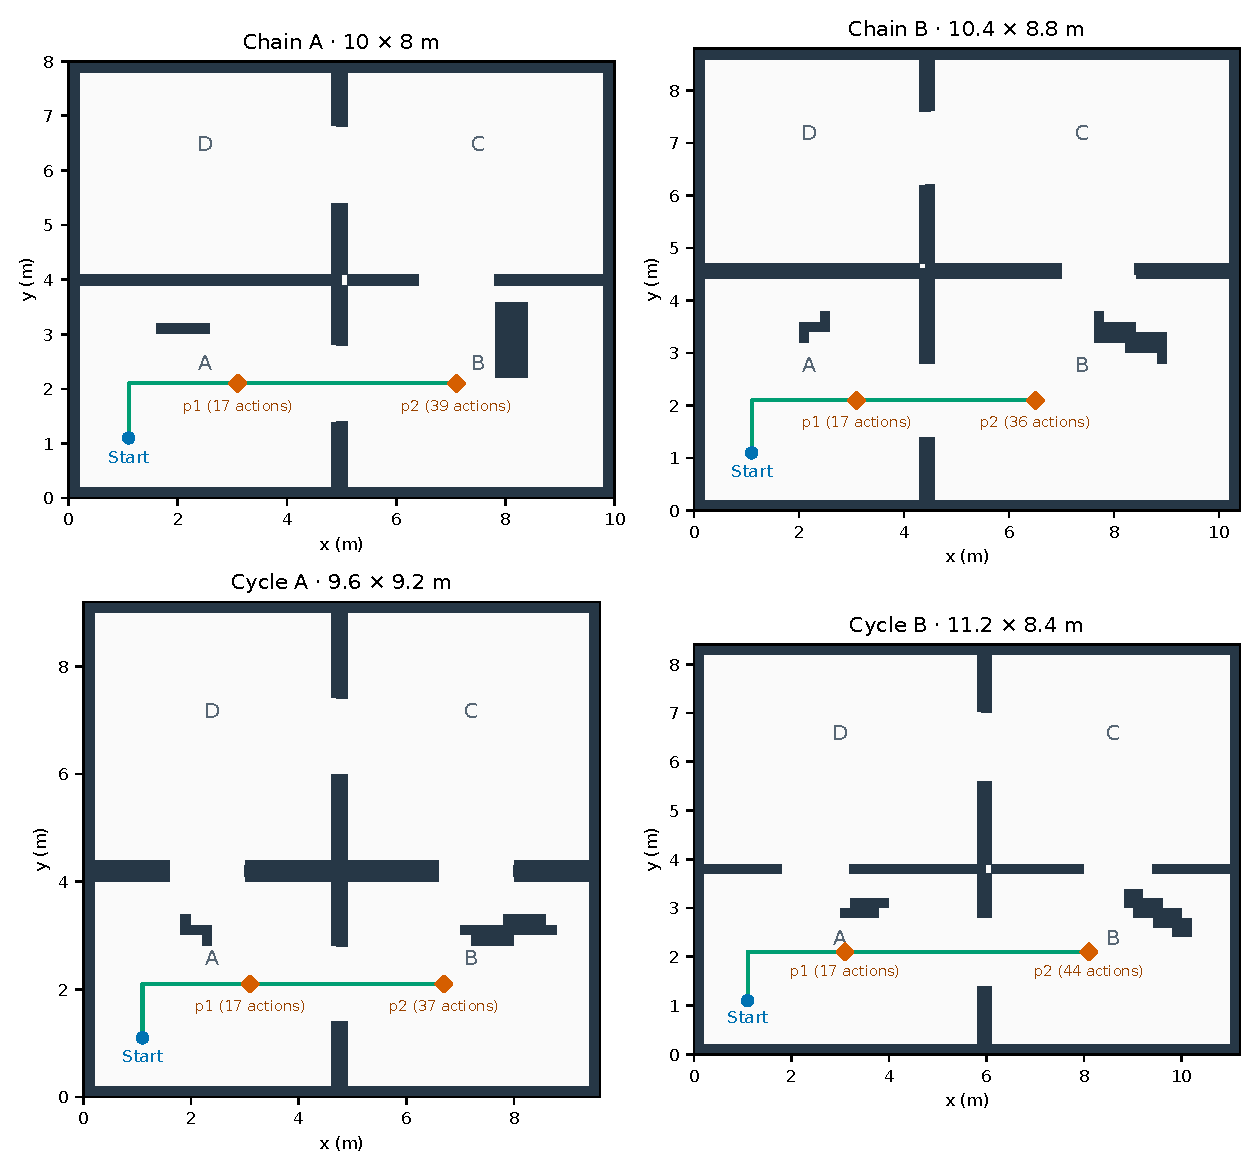
\includegraphics[width=\linewidth]{figures/b11_layouts.pdf}
\caption{The four source layouts frozen before new scores and outcomes: two chain and two cycle room graphs. Furniture CAD assets are reused, while dimensions, doors, placements, and orientations differ. This complete source map is used for generation/evaluation, not supplied to the actor. The drawn p1 markers are the original 17-action preparation checkpoints; the actual Chain~A/B p1 states advance along the same frozen script to 24/20 paid actions under the cost-only amendment, while the other six states are unchanged. The motion graph and reference denominator use the finite-radius robot. Small light-transmitting wall junctions remain part of the frozen source geometry and do not create robot-traversable room connections.}
\end{figure}
\subsection{All short-state errors and prior interventions}
\begin{table}[t]
\centering
\caption{Per-state forecast accuracy and prior sensitivity. MAE uses the same three actual gross-new object-surface areas. The neutral/category columns record whether the selected candidate changes; repeated states are not independent layouts.}
\label{tab:paired-gain-state-errors}
\begin{tabular}{llrrll}
\toprule
Layout & State & MAE V (m$^2$) & MAE A (m$^2$) & G/S V & G/S A \\
\midrule
chain\_a & p1 & 0.533 & 0.501 & 0/0 & 0/0 \\
chain\_a & p2 & 0.316 & 0.548 & 2/2 & 2/2 \\
chain\_b & p1 & 0.215 & 0.229 & 0/0 & 0/0 \\
chain\_b & p2 & 0.201 & 0.186 & 2/2 & 2/2 \\
cycle\_a & p1 & 0.228 & 0.339 & 2/2 & 2/2 \\
cycle\_a & p2 & 0.427 & 0.552 & 0/0 & 0/0 \\
cycle\_b & p1 & 1.583 & 1.170 & 7/7 & 7/7 \\
cycle\_b & p2 & 0.183 & 1.551 & 2/2 & 10/10 \\
\bottomrule
\end{tabular}
\end{table}

\begin{figure}[!htbp]\centering
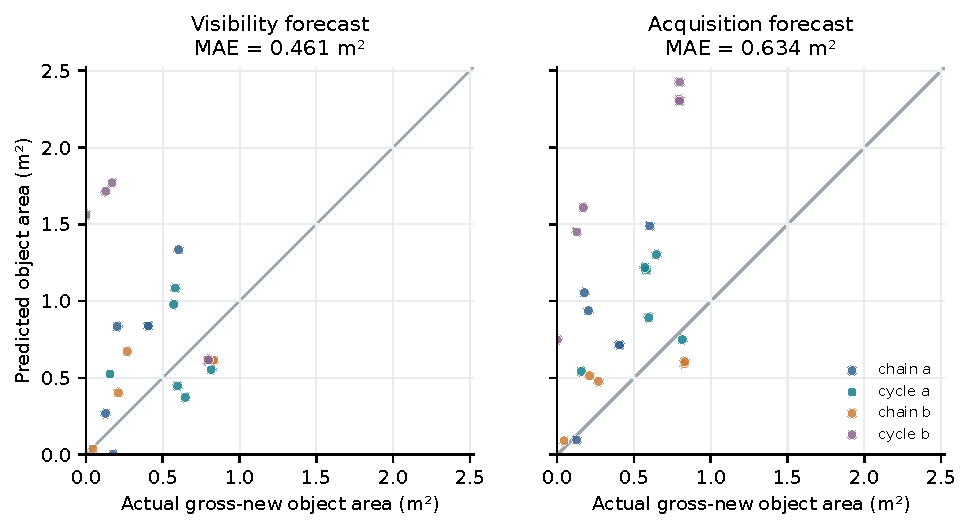
\includegraphics[width=\linewidth]{figures/b11_forecast_vs_actual.pdf}
\caption{Both category-prior forecasts against the same twenty-four measured object-gross branch outcomes in four layouts. Geometry is fitted only from each acquired prefix and the full bank and original quadrature are shared. The diagonal denotes exact prediction. The three large Cycle~B outliers are dependent branches of its second checkpoint; they dominate the net aggregate MAE increase. The points do not constitute twenty-four independent scenes.}
\end{figure}
\begin{figure}[!htbp]\centering
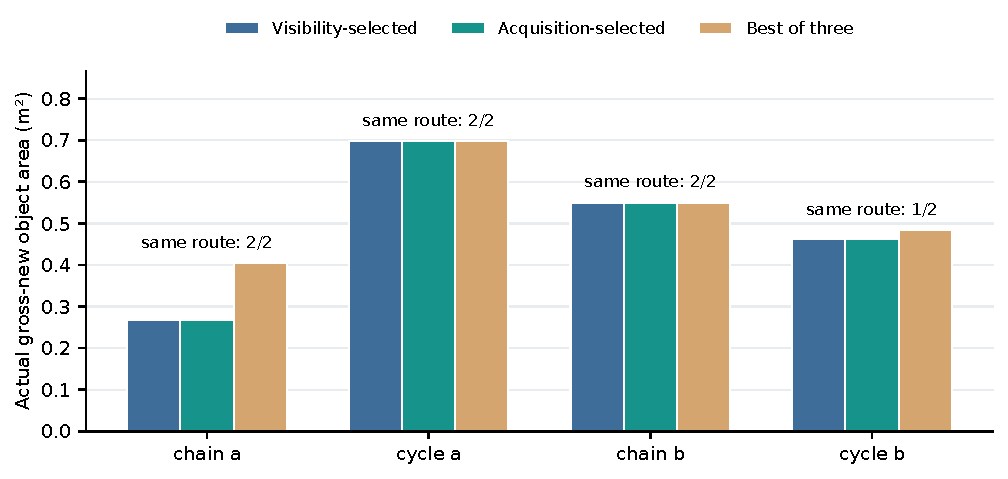
\includegraphics[width=\linewidth]{figures/b11_selected_actual_area.pdf}
\caption{Actual gross-new object surface of the two forecast-selected routes and best of the three measured candidates, averaged equally over two states per layout. The observed change in Cycle~B is only two source-reference points at one state and is accompanied by lower object net area. The other seven state selections tie.}
\end{figure}
\subsection{All complete-policy metrics and computational costs}
All episodes use 256 paid actions and return without simulated collision. Chain~B remains below 95\% under both forecasts; acquisition also misses full coverage in Chain~A. A95's finite paired differences cover only three layouts and A100's only two; no all-layout action-mean claim discards the censored cases. Three complete action traces and native meshes coincide pairwise, although their global decision records need not coincide.
\begin{table}[t]
\centering
\caption{Known, correctly free and falsely occupied fractions of the fixed start-reachable robot-free reference cells, in percent. A cell classified occupied is known but does not count as correct free coverage.}
\small\setlength{\tabcolsep}{4pt}
\begin{tabular}{llrrr}
\toprule
Layout & Arm & Known & Correct free & False occupied \\
\midrule
chain\_a & V & 100.00 & 100.00 & 0.00 \\
chain\_a & A & 99.27 & 99.27 & 0.00 \\
cycle\_a & V & 100.00 & 100.00 & 0.00 \\
cycle\_a & A & 100.00 & 100.00 & 0.00 \\
chain\_b & V & 92.40 & 92.40 & 0.00 \\
chain\_b & A & 92.40 & 92.40 & 0.00 \\
cycle\_b & V & 100.00 & 100.00 & 0.00 \\
cycle\_b & A & 100.00 & 100.00 & 0.00 \\
\bottomrule
\end{tabular}
\end{table}

\begin{table}[t]
\centering
\caption{Every prescribed complete-policy object-recall outcome. All entries are percent source-reference recall at the stated distance. Shelf and cabinet refer to the two fixed modeled instances; these are reconstruction completeness measures, not object precision or semantic classification accuracy.}
\small\setlength{\tabcolsep}{4pt}
\begin{tabular}{llrrrrr}
\toprule
Layout & Arm & Shelf 5\,cm & Shelf 10\,cm & Cabinet 5\,cm & Cabinet 10\,cm & Macro 5\,cm \\
\midrule
chain\_a & V & 79.47 & 87.51 & 81.14 & 87.39 & 80.30 \\
chain\_a & A & 80.59 & 87.99 & 69.74 & 75.00 & 75.17 \\
cycle\_a & V & 64.93 & 80.44 & 91.03 & 97.74 & 77.98 \\
cycle\_a & A & 64.93 & 80.44 & 91.03 & 97.74 & 77.98 \\
chain\_b & V & 79.77 & 85.09 & 95.45 & 97.98 & 87.61 \\
chain\_b & A & 79.77 & 85.09 & 95.45 & 97.98 & 87.61 \\
cycle\_b & V & 79.85 & 87.86 & 95.67 & 98.30 & 87.76 \\
cycle\_b & A & 79.85 & 87.86 & 95.67 & 98.30 & 87.76 \\
\bottomrule
\end{tabular}
\end{table}

\begin{table}[t]
\centering
\caption{Whole-scene native TSDF metrics for all eight prescribed episodes, in percent. Fixed independently sampled source references and the original native area sampler are used without post-hoc registration.}
\small\setlength{\tabcolsep}{4pt}
\begin{tabular}{llrrrrrr}
\toprule
Layout & Arm & $P_5$ & $R_5$ & $F_{1,5}$ & $P_{10}$ & $R_{10}$ & $F_{1,10}$ \\
\midrule
chain\_a & V & 99.38 & 98.96 & 99.17 & 99.97 & 99.35 & 99.66 \\
chain\_a & A & 99.41 & 97.99 & 98.69 & 100.00 & 98.46 & 99.23 \\
cycle\_a & V & 99.83 & 98.94 & 99.38 & 100.00 & 99.48 & 99.74 \\
cycle\_a & A & 99.83 & 98.94 & 99.38 & 100.00 & 99.48 & 99.74 \\
chain\_b & V & 99.84 & 85.80 & 92.29 & 100.00 & 87.53 & 93.35 \\
chain\_b & A & 99.84 & 85.80 & 92.29 & 100.00 & 87.53 & 93.35 \\
cycle\_b & V & 99.58 & 97.73 & 98.65 & 100.00 & 98.62 & 99.30 \\
cycle\_b & A & 99.58 & 97.73 & 98.65 & 100.00 & 98.62 & 99.30 \\
\bottomrule
\end{tabular}
\end{table}

\begin{table}[t]
\centering
\caption{Complete recorded execution and computation costs. Decisions include local action requests and global selection. Wall times are measured with up to three concurrent single-library-thread processes; they are not logical action durations, robot travel times, isolated latency, or real-time guarantees.}
\small\setlength{\tabcolsep}{4pt}
\begin{tabular}{llrrrrr}
\toprule
Layout & Arm & Paid actions & Global calls & Decision wall (s) & Total wall (s) & Collisions \\
\midrule
chain\_a & V & 256 & 29 & 244.7 & 395.0 & 0 \\
chain\_a & A & 256 & 32 & 1483.8 & 1638.0 & 0 \\
cycle\_a & V & 256 & 28 & 228.1 & 384.0 & 0 \\
cycle\_a & A & 256 & 28 & 1761.2 & 1921.3 & 0 \\
chain\_b & V & 256 & 28 & 203.5 & 353.1 & 0 \\
chain\_b & A & 256 & 13 & 1282.2 & 1432.9 & 0 \\
cycle\_b & V & 256 & 13 & 104.8 & 245.1 & 0 \\
cycle\_b & A & 256 & 14 & 960.9 & 1098.1 & 0 \\
\bottomrule
\end{tabular}
\end{table}

The acquired-frame ledger has 257 receipts per complete episode, including bootstrap. Source/evaluator hashes, posterior recomputation, actual pose/return records, final correct-free belief, and all native metrics are independently checked. Frame receipt chains are verified rather than all raw frame values being reread. Zero computation fallbacks or interrupted attempts occur in this matrix. Source and metric receipts, the per-track error decomposition, all candidate records, and editable CSV data are retained in the experiment bundle. The CPU cost and exact cache/process-snapshot equivalence tests are implementation evidence, not improved scientific outcomes or a real-time guarantee.
